\documentclass{article}

\usepackage{amsmath}
\usepackage{amssymb}

\usepackage{booktabs}
\usepackage{float}
\usepackage{colortbl}
\usepackage{xcolor}

\usepackage{a4wide}
\usepackage{setspace}
\usepackage{geometry}
\usepackage{pdflscape}
\usepackage{parskip}
\doublespacing
\geometry{margin=1.5in}

\usepackage{graphicx}
\graphicspath{ {../figures/} }

\usepackage{hyperref}
\hypersetup{
	colorlinks = true,
	linkcolor = black,
	urlcolor=blue
}

\author{Patrick Massey and Elliott Metzler}
\title{Causal Recreational Cannabis}
\date{5/13/2022}

\begin{document}
\maketitle

\begin{abstract}

Can legalizing the recreational use of cannabis reduce rates of drug poisoning deaths? This paper seeks to study the relationship between changes in state-level policy toward recreational cannabis use and drug poisoning death rates. Specifically, we evaluate the impact of such policy change on the first state to legalize, Colorado. We implement a synthetic control design in which we use demographic data for each state in the United States, including Washington D.C., and estimate the causal impact of Colorado's legalization policy shift in 2012. We find [[insert findings and explanation of implications]].

\end{abstract}

\newpage

\section{Introduction and Background}

[[Need to do]]

\begin{table}[H]

\caption{\label{tab:tab:rollout}Marijuana Legalization by State}
\centering
\begin{tabular}[t]{lr}
\toprule
State & Year\\
\midrule
\cellcolor{gray!6}{Colorado} & \cellcolor{gray!6}{2012}\\
Washington & 2012\\
\cellcolor{gray!6}{Alaska} & \cellcolor{gray!6}{2014}\\
Oregon & 2014\\
\cellcolor{gray!6}{California} & \cellcolor{gray!6}{2016}\\
\addlinespace
Maine & 2016\\
\cellcolor{gray!6}{Massachusetts} & \cellcolor{gray!6}{2016}\\
Nevada & 2016\\
\cellcolor{gray!6}{Michigan} & \cellcolor{gray!6}{2018}\\
Vermont & 2018\\
\bottomrule
\end{tabular}
\end{table}


Figure \ref{fig:death_rates_trend} shows the average death rate across the United States and the average death rate for Colorado between 2000 and 2018.

\begin{figure}[H]
	\begin{center}
		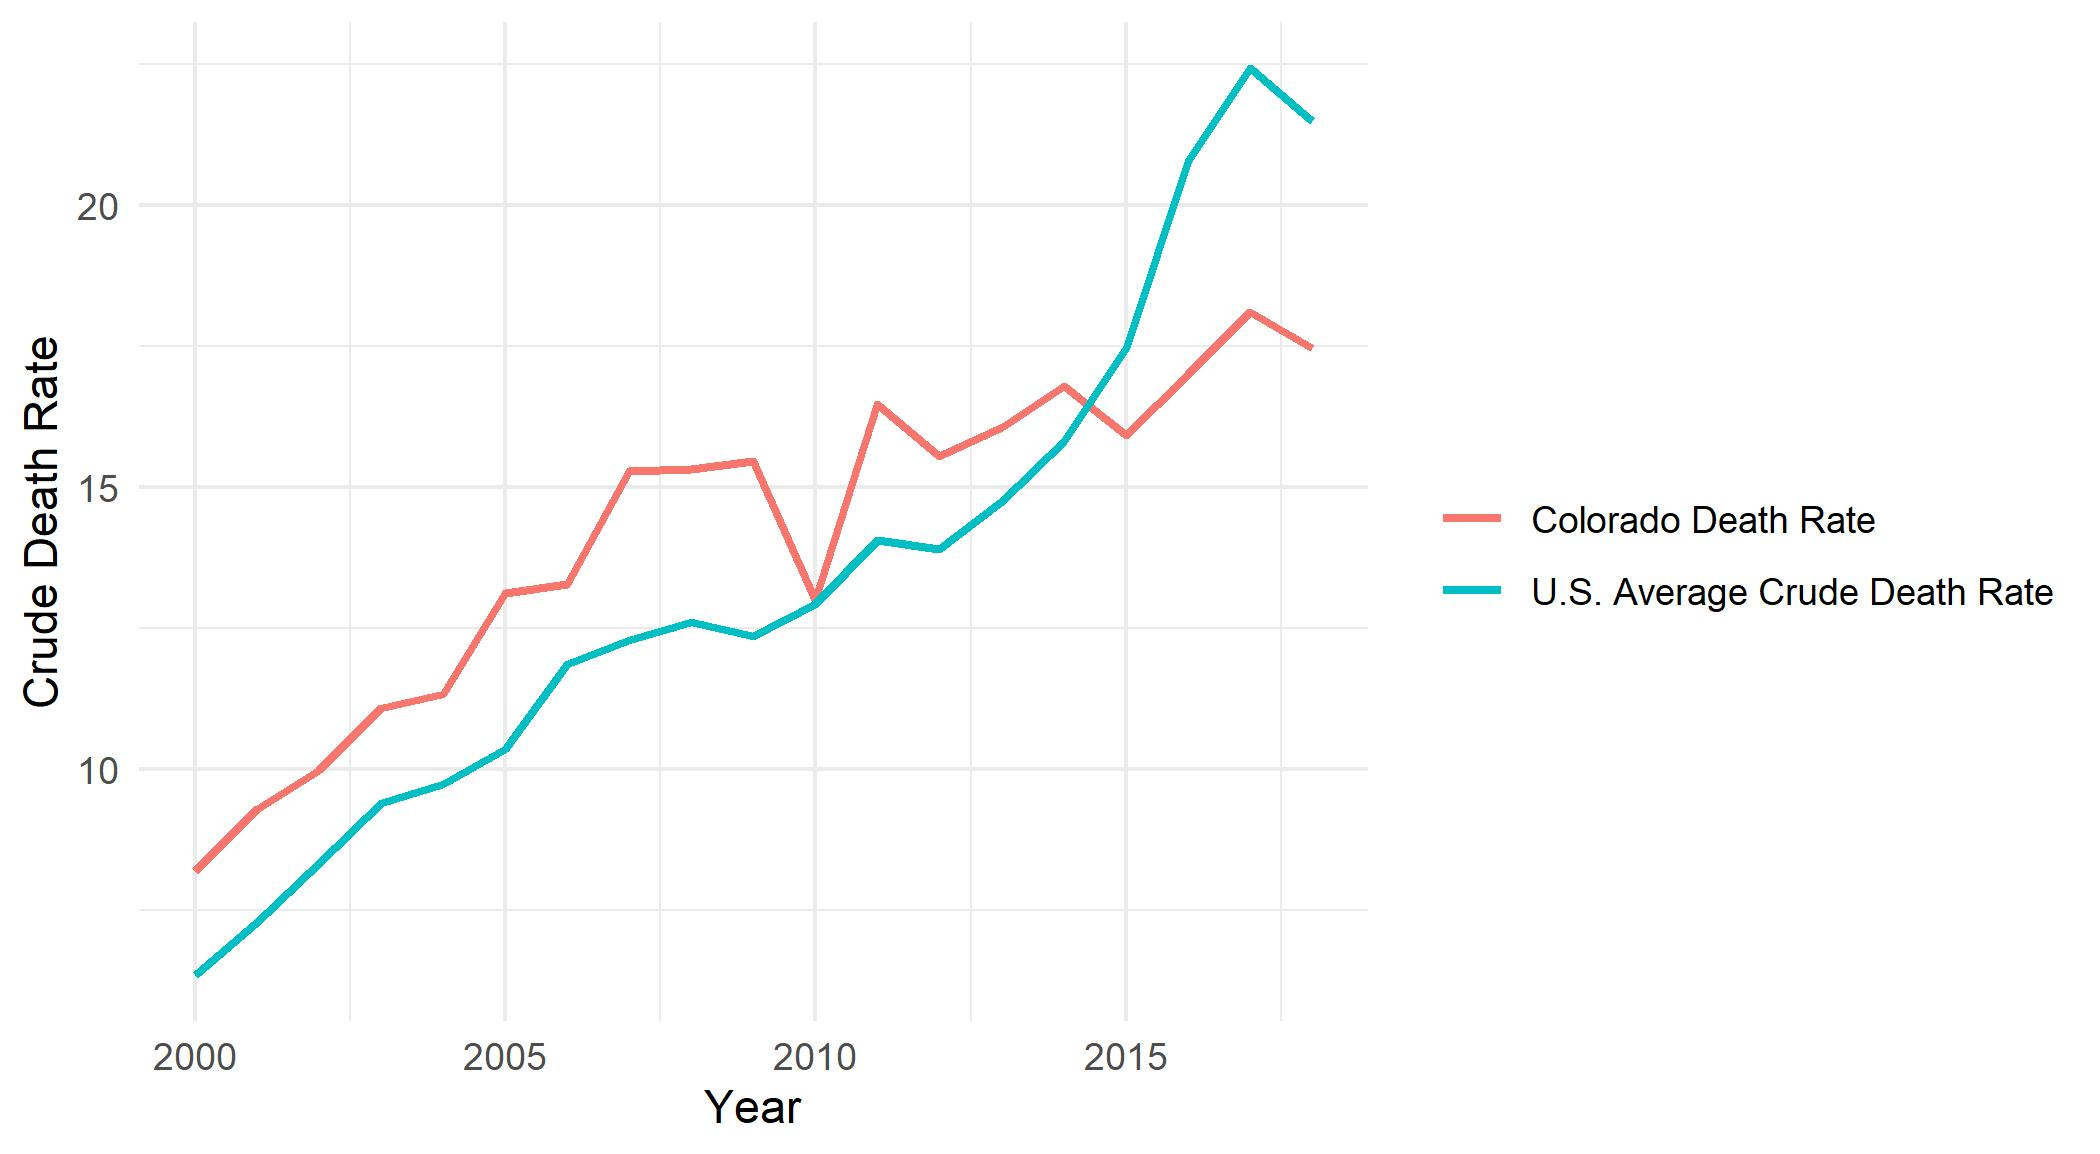
\includegraphics[width=0.85\textwidth]{death_rates_trend}
	\end{center}
	\caption{Drug Poisoning Death Rates Trend (2000-2018)}
	\label{fig:death_rates_trend}
\end{figure}

\section{Data}

The data employed for this paper originates from two sources. First, we source data on drug poisoning deaths, population, and an estimate of the crude drug poisoning death rate from the United States Center for Disease Control (``CDC''). Second, we source state-level demographic data from IPUMS USA, which is a database harmonizing, organizing, and structuring data from various population surveys in the United States over time.

The first data set contains summary statistics by state and by year from 1999 to 2018. For each state in each year, the data reports the number of deaths due to drug poisoning, the population, and the ratio of the two previous variables as the crude death rate. Additionally, this data reports an estimate of the standard error for the crude death rate, and a lower and upper confidence interval around the point estimate. In addition to these base estimates, the data originally includes age-adjusted rates with standard errors and confidence intervals and the United State-wide crude death rate and United State-wide age-adjusted death rate. 

From this data set, we focus on the crude death rate for the state and extract this variable along with the state and year variables for data merging purposes. We focus our attention on the crude death rate statistic for a couple of important reasons. First, using the death rate as opposed to the total number of deaths allows us to immediately control for differences in state population when estimating our model. Second, we exclude the age-adjusted rate because our model also accounts for age demographics explicitly as covariates, so it would be inappropriate to use this as our outcome variable of interest.

The second data set contains nearly 28 million entries where each entry represents a person included in [[a survey]] in a particular year.  Importantly, this data includes the year and state in which that entry resided along with extensive demographic data. Thus, we are able to use the groups of these entries associated with each year and each state and calculate demographic summary information representative of each year in each state. We include in our demographic summaries the proportion of the population that is listed as male as compared to female [[should footnote simplicity of coding here ( I don't remember seeing info about non-binary or choose not to identify)]], a summary of a few significant age buckets, proportions of the population based on race, on marital status, on education, and on employment status. Additionally, we summarize the mean number of hours worked, the median income, the mean number of children, and the mean number of children under 5 years old. We present the mean and standard deviation of each of these demographic variables in Table \ref{tab:var_summary}.

To construct our final data set for use in analysis, we combine the two data sources. Since we have summarized the latter data set at the state and year level and the first data set is already at this level, we merge on the state and year. Thus, we have data for each state, inclusive of Washington D.C., for each year between 2000 and 2018 with data on deaths associated with drug poisoning, population, crude death rate, and all of our descriptive demographics data.

\begin{table}[H]

\caption{\label{tab:tab:var_summary}Variable Summary}
\centering
\begin{tabular}[t]{lrr}
\toprule
Variable & Mean & Std. Dev\\
\midrule
\addlinespace[0.3em]
\multicolumn{3}{l}{\textbf{Drug Poisonings}}\\
\hspace{1em}\cellcolor{gray!6}{Deaths} & \cellcolor{gray!6}{777.179} & \cellcolor{gray!6}{887.743}\\
\hspace{1em}Population & 5995451.840 & 6730237.227\\
\hspace{1em}\cellcolor{gray!6}{Crude Death Rate} & \cellcolor{gray!6}{13.381} & \cellcolor{gray!6}{7.082}\\
\addlinespace[0.3em]
\multicolumn{3}{l}{\textbf{Gender Population Proportions}}\\
\hspace{1em}Male & 0.489 & 0.012\\
\hspace{1em}\cellcolor{gray!6}{Female} & \cellcolor{gray!6}{0.511} & \cellcolor{gray!6}{0.012}\\
\addlinespace[0.3em]
\multicolumn{3}{l}{\textbf{Age Population Proportions}}\\
\hspace{1em}Under 30 & 0.176 & 0.022\\
\hspace{1em}\cellcolor{gray!6}{Under 50} & \cellcolor{gray!6}{0.450} & \cellcolor{gray!6}{0.042}\\
\hspace{1em}Over 50 & 0.374 & 0.045\\
\addlinespace[0.3em]
\multicolumn{3}{l}{\textbf{Race Population Proportions}}\\
\hspace{1em}\cellcolor{gray!6}{American Indian} & \cellcolor{gray!6}{0.018} & \cellcolor{gray!6}{0.039}\\
\hspace{1em}Asian & 0.039 & 0.070\\
\hspace{1em}\cellcolor{gray!6}{Black} & \cellcolor{gray!6}{0.088} & \cellcolor{gray!6}{0.094}\\
\hspace{1em}Other Race & 0.045 & 0.039\\
\hspace{1em}\cellcolor{gray!6}{White} & \cellcolor{gray!6}{0.810} & \cellcolor{gray!6}{0.131}\\
\addlinespace[0.3em]
\multicolumn{3}{l}{\textbf{Marital Status Population Proportions}}\\
\hspace{1em}Married & 0.609 & 0.062\\
\hspace{1em}\cellcolor{gray!6}{Not Married} & \cellcolor{gray!6}{0.391} & \cellcolor{gray!6}{0.062}\\
\addlinespace[0.3em]
\multicolumn{3}{l}{\textbf{Education Population Proportions}}\\
\hspace{1em}Less High School & 0.084 & 0.029\\
\hspace{1em}\cellcolor{gray!6}{High School} & \cellcolor{gray!6}{0.372} & \cellcolor{gray!6}{0.050}\\
\hspace{1em}Some College & 0.247 & 0.036\\
\hspace{1em}\cellcolor{gray!6}{College} & \cellcolor{gray!6}{0.191} & \cellcolor{gray!6}{0.034}\\
\hspace{1em}Higher College & 0.106 & 0.041\\
\addlinespace[0.3em]
\multicolumn{3}{l}{\textbf{Employment Population Proportions and Summary Statistics}}\\
\hspace{1em}\cellcolor{gray!6}{Employed} & \cellcolor{gray!6}{0.724} & \cellcolor{gray!6}{0.045}\\
\hspace{1em}Not Employed & 0.276 & 0.045\\
\hspace{1em}\cellcolor{gray!6}{Mean Hrs Worked} & \cellcolor{gray!6}{32.222} & \cellcolor{gray!6}{2.269}\\
\hspace{1em}Median Income & 22380.650 & 5043.007\\
\addlinespace[0.3em]
\multicolumn{3}{l}{\textbf{Children Summary Statistics}}\\
\hspace{1em}\cellcolor{gray!6}{Mean Children} & \cellcolor{gray!6}{0.823} & \cellcolor{gray!6}{0.107}\\
\hspace{1em}Mean Children Under 5 years old & 0.168 & 0.029\\
\bottomrule
\end{tabular}
\end{table}


Please see the appendix for detailed descriptions of our procedure to re-code and summarize variables.

\section{Methodology}

We utilize the synthetic control method first developed by Abadie and Gardeazabal (2003) and then expanded upon in Abadie et. al (2010)(2015). Similar to Abadie et. al (2010) we are analyzing the impact of a government policy shock. In this analysis we are estimating the impact of Colorado's legalization of recreation cannabis in 2012. For our synthetic control, Colorado is the treatment state of interest, and we have a donor pool of 41[Need to double check that's correct] states. The synthetic control method [MORE INFO HERE]

Suppose that we have $1,2...S+1$ states and let $s = 1$ be the treated state, additionally we have $t = 1,2...T$ time periods where $T_0$ represents the number of pretreatment periods, and $T_0 + 1...T$ are the posttreatment periods. With that let $Y_{st}$ be the crude death rate for state $s$ at time $t$. In a posttreatment time line we are estimating
\begin{equation*}
\hat{\alpha} = Y_{1t} - \sum_{s=2}^{S+1}w^{*}Y_{st}
\end{equation*}
$w^{*}_s$ is a vector of optimally chosen weights for states from our donor pool to represent our synthetic Colorado. Again deriving from Abadie (2010) $w^{*}_s$ is the vector of weights that minimizes the following equation
\begin{equation*}
(X_1 - X_0w)'V(X_1 - X_0w)
\end{equation*}
$X_1$ is a $(K \times 1)$ vector of state population variables and $X_0$ is a $(K \times S)$ matrix of state population variables for $S$ donor states. Note that $w_s \geq 0$ and $\sum w_s = 1$.

We utilize the weights generated to create a synthetic Colorado, where we examine the counterfactual of a Colorado that never legalized recreational cannabis. Additionally we follow Abadie (2010) and use their placebo technique as a robustness check. The placebo technique consists of assigning each state in our donor pool as the treated state and then creating an optimal $w^{*}_s$, from the other donor states as well as the treated state, in the pretreatment period. Utilizing the weights we calculate the posttreatment root mean squared prediction error (RMSPE) for each state. We then take a ratio between the post/pretreatment RMSPE for each state. We expect this value to be high for our treated state, which would suggest that the posttreatment RMSPE is large due to the differences between the synthetic and the observed Colorado.

\begin{table}[H]

\caption{\label{tab:unit_weight_table_colorado}Synthetic Weights}
\centering
\begin{tabular}[t]{lr}
\toprule
Unit & Weight\\
\midrule
\cellcolor{gray!6}{Alabama} & \cellcolor{gray!6}{0.0000000}\\
Arizona & 0.4537880\\
\cellcolor{gray!6}{Arkansas} & \cellcolor{gray!6}{0.0000000}\\
Connecticut & 0.0000016\\
\cellcolor{gray!6}{Delaware} & \cellcolor{gray!6}{0.0000000}\\
\addlinespace
District of Columbia & 0.0946779\\
\cellcolor{gray!6}{Florida} & \cellcolor{gray!6}{0.0000000}\\
Georgia & 0.0000000\\
\cellcolor{gray!6}{Hawaii} & \cellcolor{gray!6}{0.0000001}\\
Idaho & 0.0000000\\
\addlinespace
\cellcolor{gray!6}{Illinois} & \cellcolor{gray!6}{0.0000000}\\
Indiana & 0.0000000\\
\cellcolor{gray!6}{Iowa} & \cellcolor{gray!6}{0.0000000}\\
Kansas & 0.0000001\\
\cellcolor{gray!6}{Kentucky} & \cellcolor{gray!6}{0.0000000}\\
\addlinespace
Louisiana & 0.0000000\\
\cellcolor{gray!6}{Maryland} & \cellcolor{gray!6}{0.0000000}\\
Minnesota & 0.0000603\\
\cellcolor{gray!6}{Mississippi} & \cellcolor{gray!6}{0.0000000}\\
Missouri & 0.0000000\\
\addlinespace
\cellcolor{gray!6}{Montana} & \cellcolor{gray!6}{0.0000000}\\
Nebraska & 0.0000001\\
\cellcolor{gray!6}{New Hampshire} & \cellcolor{gray!6}{0.3754123}\\
New Jersey & 0.0000001\\
\cellcolor{gray!6}{New Mexico} & \cellcolor{gray!6}{0.0000000}\\
\addlinespace
New York & 0.0000000\\
\cellcolor{gray!6}{North Carolina} & \cellcolor{gray!6}{0.0000000}\\
North Dakota & 0.0000005\\
\cellcolor{gray!6}{Ohio} & \cellcolor{gray!6}{0.0000000}\\
Oklahoma & 0.0000000\\
\addlinespace
\cellcolor{gray!6}{Pennsylvania} & \cellcolor{gray!6}{0.0000000}\\
Rhode Island & 0.0000000\\
\cellcolor{gray!6}{South Carolina} & \cellcolor{gray!6}{0.0000000}\\
South Dakota & 0.0000000\\
\cellcolor{gray!6}{Tennessee} & \cellcolor{gray!6}{0.0000000}\\
\addlinespace
Texas & 0.0000005\\
\cellcolor{gray!6}{Utah} & \cellcolor{gray!6}{0.0760580}\\
Virginia & 0.0000001\\
\cellcolor{gray!6}{West Virginia} & \cellcolor{gray!6}{0.0000000}\\
Wisconsin & 0.0000000\\
\addlinespace
\cellcolor{gray!6}{Wyoming} & \cellcolor{gray!6}{0.0000000}\\
\bottomrule
\end{tabular}
\end{table}


\begin{table}[H]

\caption{\label{tab:balance_table_colorado}Balance Table}
\centering
\begin{tabular}[t]{lrrr}
\toprule
Variable & Colorado & Synthetic Colorado & Donor Sample\\
\midrule
\cellcolor{gray!6}{American Indian Proportion} & \cellcolor{gray!6}{0.009} & \cellcolor{gray!6}{0.022} & \cellcolor{gray!6}{0.014}\\
Asian Proportion & 0.026 & 0.025 & 0.035\\
\cellcolor{gray!6}{Black Proportion} & \cellcolor{gray!6}{0.030} & \cellcolor{gray!6}{0.059} & \cellcolor{gray!6}{0.098}\\
College Proportion & 0.245 & 0.204 & 0.184\\
\cellcolor{gray!6}{Employed Proportion} & \cellcolor{gray!6}{0.753} & \cellcolor{gray!6}{0.732} & \cellcolor{gray!6}{0.726}\\
\addlinespace
Female Proportion & 0.508 & 0.514 & 0.515\\
\cellcolor{gray!6}{Hispanic Proportion} & \cellcolor{gray!6}{0.139} & \cellcolor{gray!6}{0.120} & \cellcolor{gray!6}{0.067}\\
High School Proportion & 0.304 & 0.341 & 0.384\\
\cellcolor{gray!6}{Less Than High School Proportion} & \cellcolor{gray!6}{0.068} & \cellcolor{gray!6}{0.084} & \cellcolor{gray!6}{0.090}\\
Male Proportion & 0.492 & 0.486 & 0.485\\
\addlinespace
\cellcolor{gray!6}{Married Proportion} & \cellcolor{gray!6}{0.632} & \cellcolor{gray!6}{0.604} & \cellcolor{gray!6}{0.627}\\
Mean Children & 0.813 & 0.848 & 0.844\\
\cellcolor{gray!6}{Mean Children U5} & \cellcolor{gray!6}{0.183} & \cellcolor{gray!6}{0.179} & \cellcolor{gray!6}{0.174}\\
Mean Hrs Worked & 33.882 & 32.677 & 32.706\\
\cellcolor{gray!6}{Median Income} & \cellcolor{gray!6}{24523.077} & \cellcolor{gray!6}{23473.869} & \cellcolor{gray!6}{21327.955}\\
\addlinespace
More Than College Proportion & 0.130 & 0.122 & 0.100\\
\cellcolor{gray!6}{Not Employed Proportion} & \cellcolor{gray!6}{0.247} & \cellcolor{gray!6}{0.268} & \cellcolor{gray!6}{0.274}\\
Not Hispanic Proportion & 0.861 & 0.880 & 0.933\\
\cellcolor{gray!6}{Not Married Proportion} & \cellcolor{gray!6}{0.368} & \cellcolor{gray!6}{0.396} & \cellcolor{gray!6}{0.373}\\
Other Race Proportion & 0.064 & 0.056 & 0.041\\
\addlinespace
\cellcolor{gray!6}{Over 50 Proportion} & \cellcolor{gray!6}{0.337} & \cellcolor{gray!6}{0.348} & \cellcolor{gray!6}{0.360}\\
Some College Proportion & 0.253 & 0.250 & 0.242\\
\cellcolor{gray!6}{Under 30 Proportion} & \cellcolor{gray!6}{0.180} & \cellcolor{gray!6}{0.180} & \cellcolor{gray!6}{0.175}\\
Under 50 Proportion & 0.483 & 0.472 & 0.466\\
\cellcolor{gray!6}{White Proportion} & \cellcolor{gray!6}{0.870} & \cellcolor{gray!6}{0.837} & \cellcolor{gray!6}{0.813}\\
\bottomrule
\end{tabular}
\end{table}


\begin{figure}[H]
	\begin{center}
		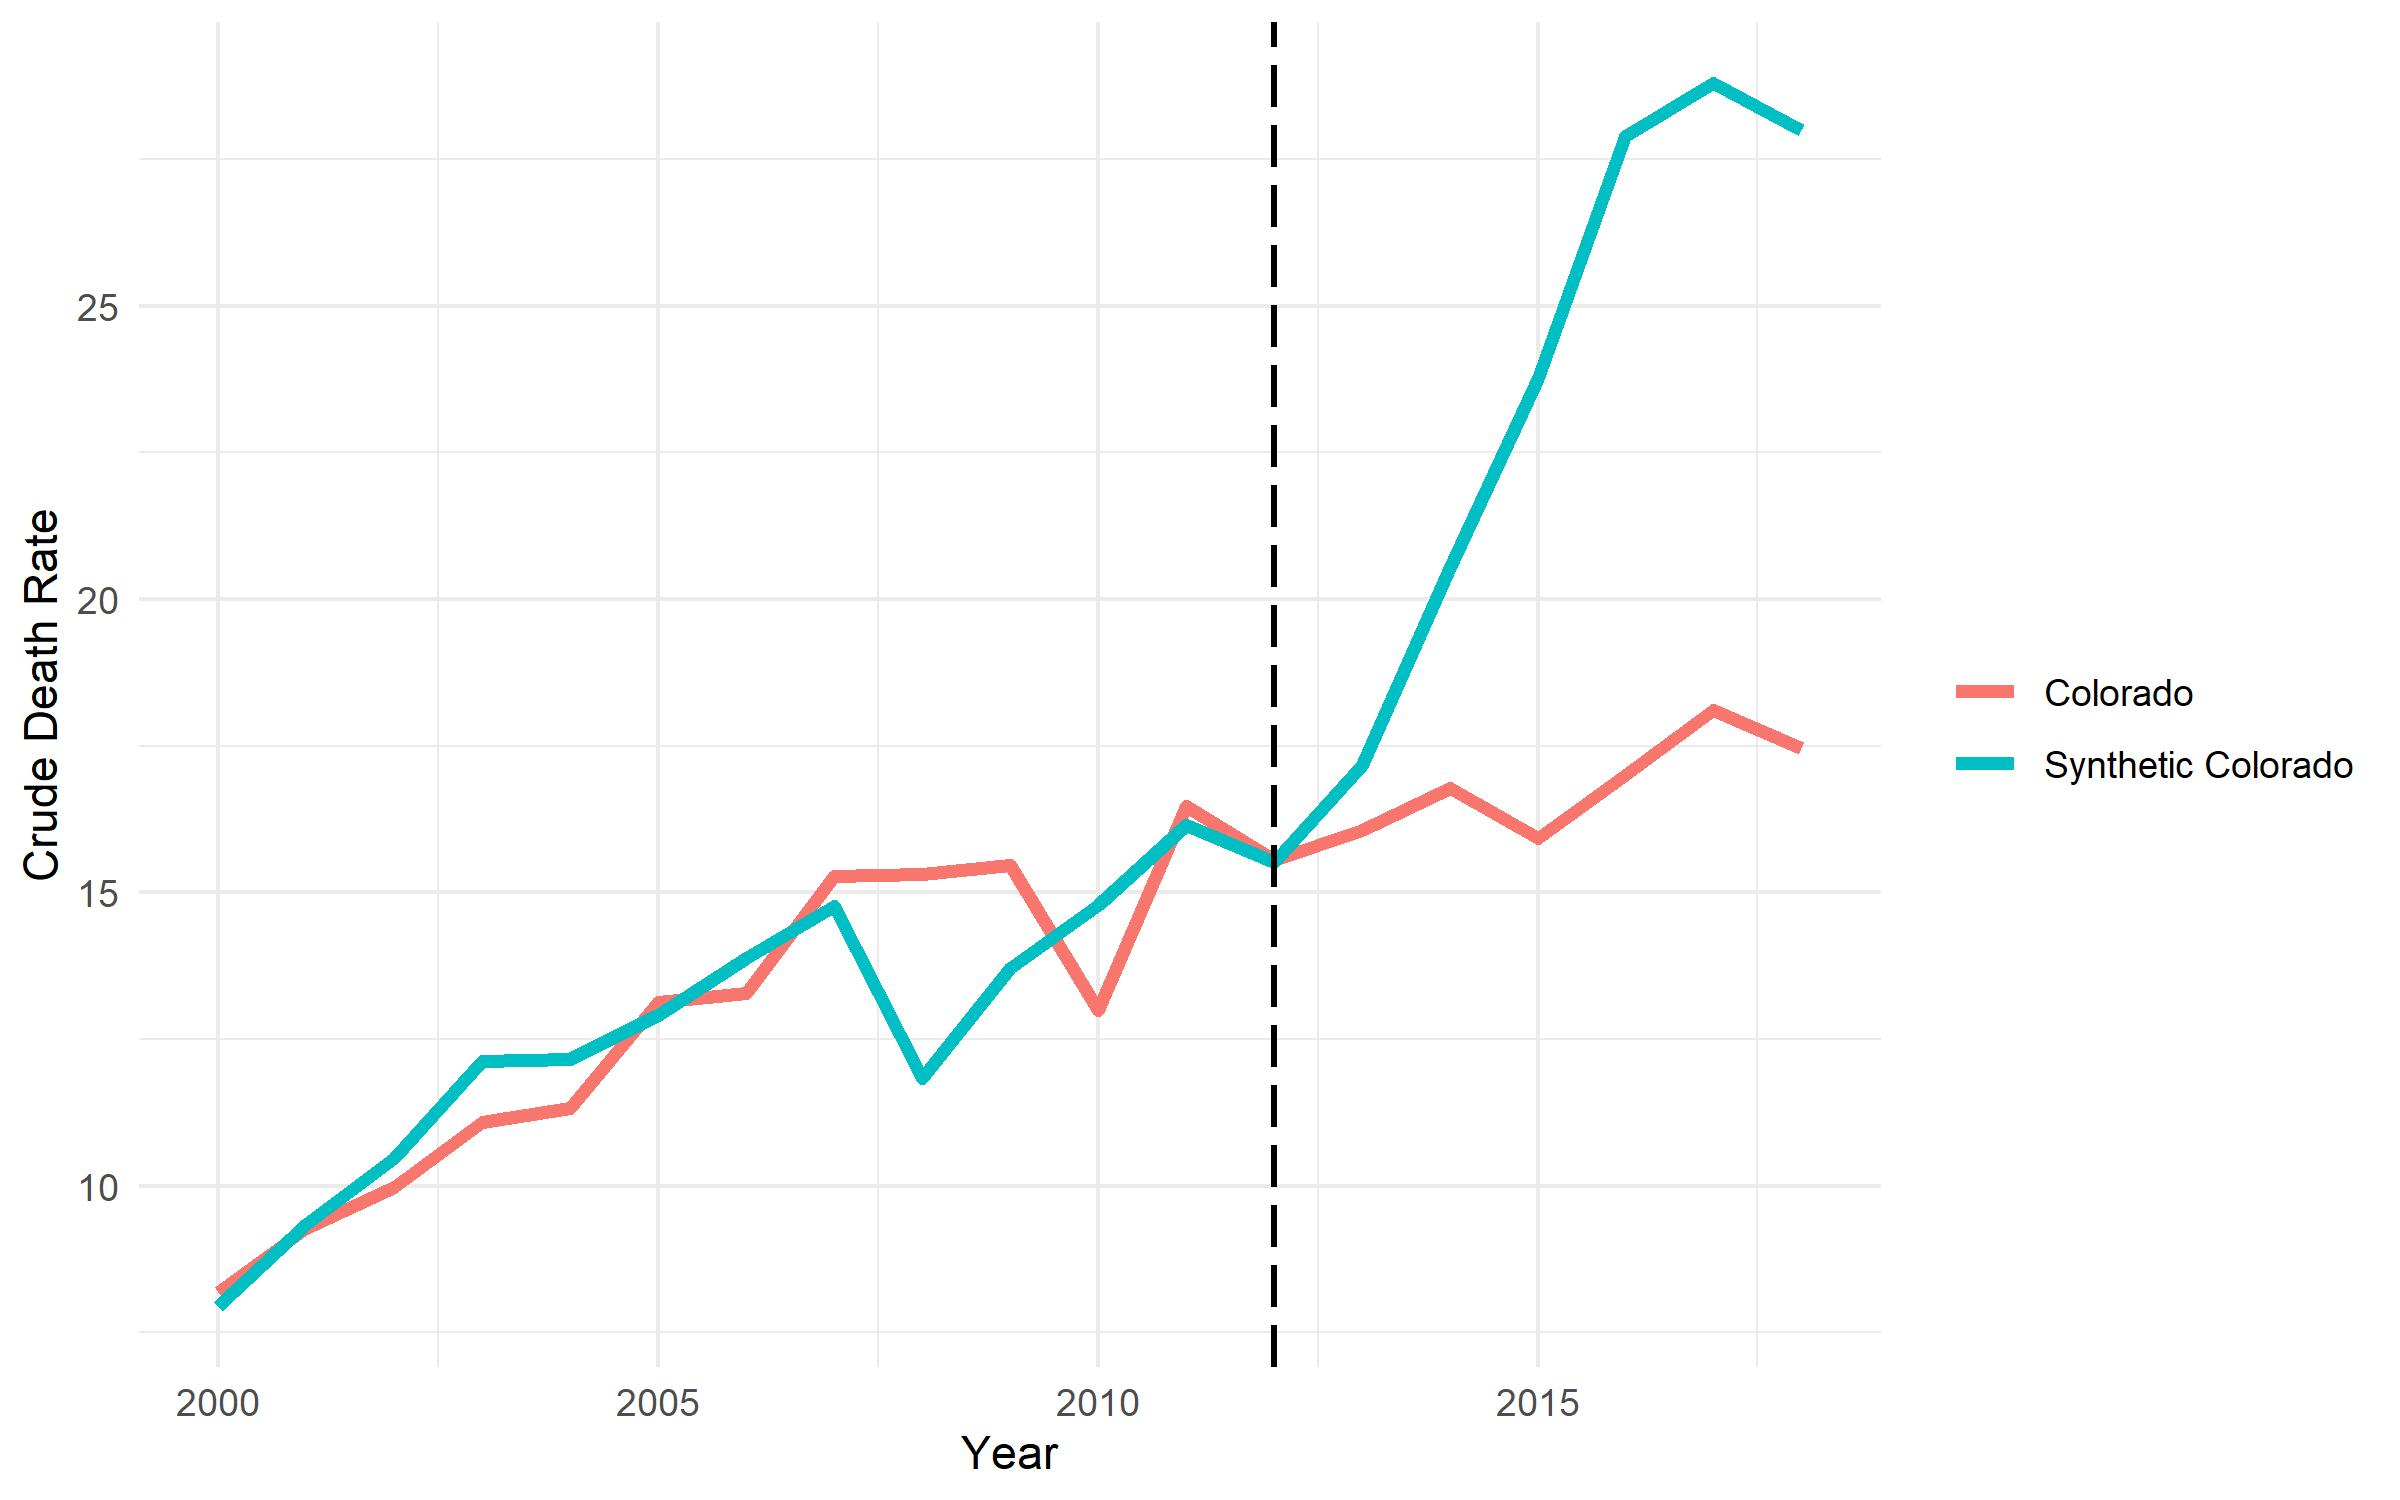
\includegraphics[width=0.85\textwidth]{trends_plot_colorado}
	\end{center}
	\caption{Trends in Crude Death Rate: Colorado vs. Synthetic Colorado}
	\label{fig:trends_plot_colorado}
\end{figure}

\begin{figure}[H]
	\begin{center}
		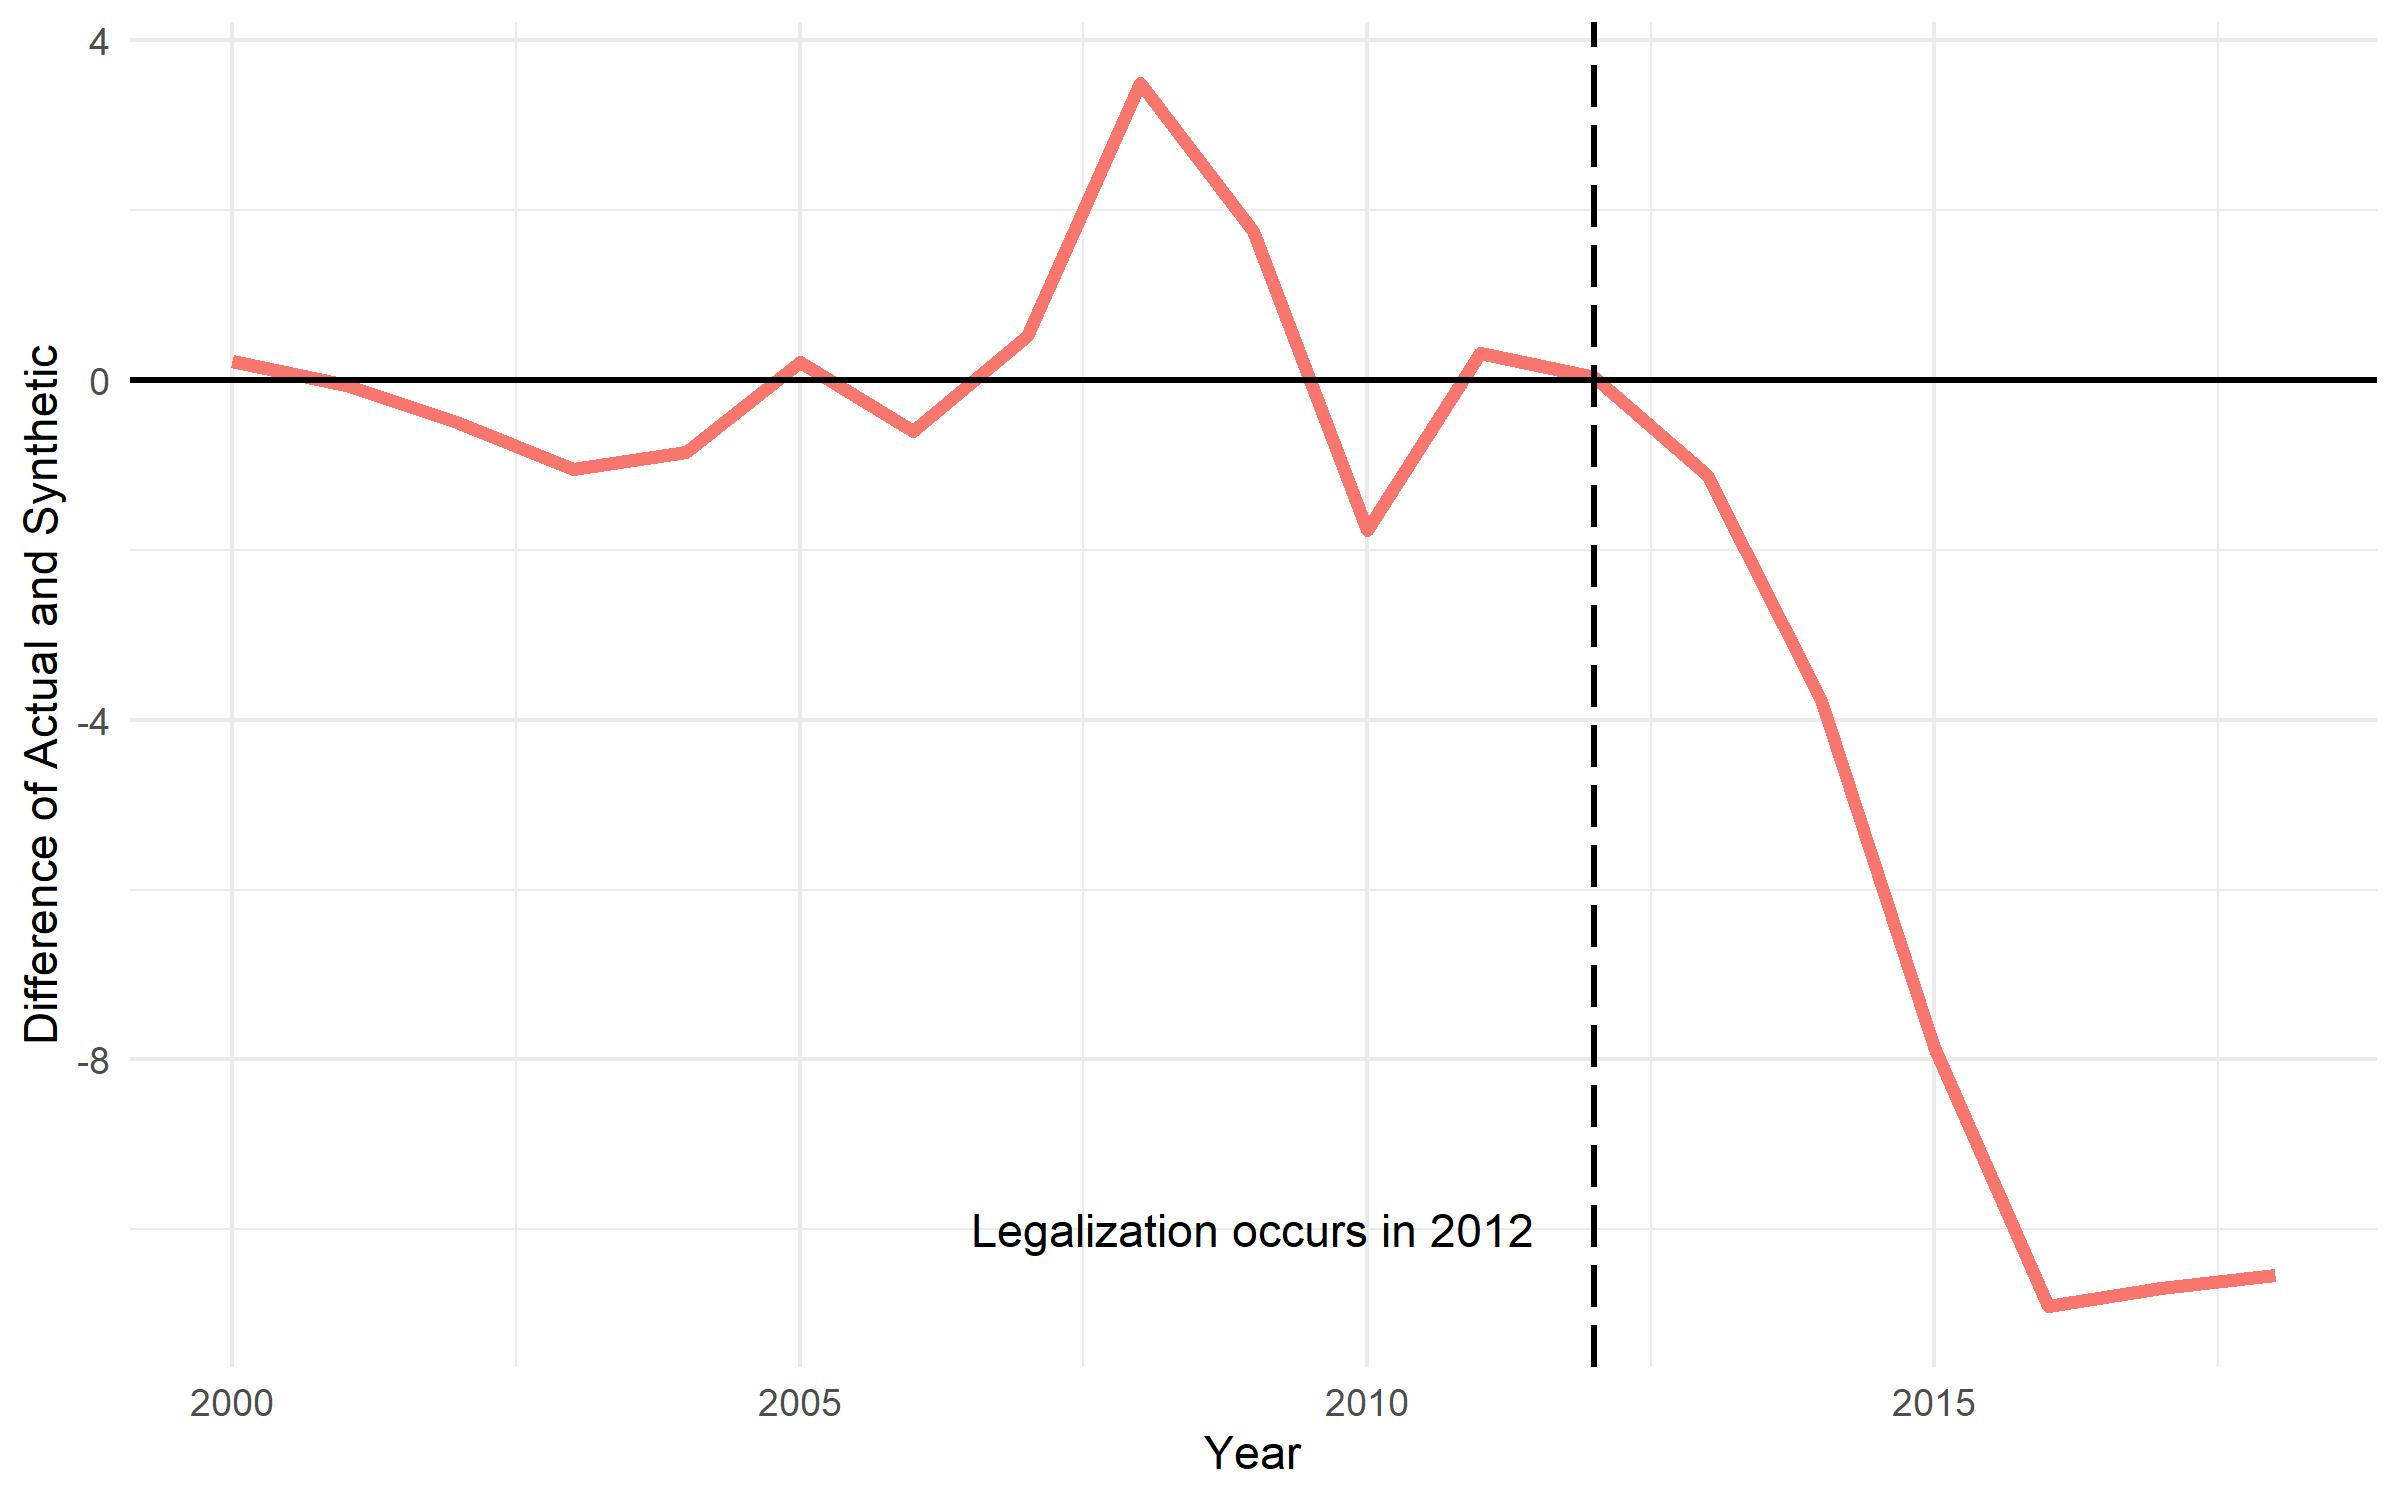
\includegraphics[width=0.85\textwidth]{diffs_plot_colorado}
	\end{center}
	\caption{Differences in Crude Death Rate: Colorado vs. Synthetic Colorado}
	\label{fig:diffs_plot_colorado}
\end{figure}


\section{Discussion}

\section{Conclusion}

\section{Appendix}

\subsection{Variable Re-coding Procedure Detail}

\begin{itemize}
\item
Gender ( \emph{sex})

Original coding:
\begin{itemize}
\item
1 = Male
\item
2 = Female
\end{itemize}
Summarized by calculating proportion of total that is male and proportion of total that is female.

\item
Age (\emph{age})

Original coding:
\begin{itemize}
\item
Actual age of entry
\end{itemize}
Summarized by categorizing into the following age groups and calculating the proportion of the total that fall into that age group.
\begin{itemize}
\item
Under 30 years old
\item
Between 30 years old and under 50 years old
\item
Over 50 years old
\end{itemize}

\item
Need to do - finish transferring notes from the markdown file into here.

\end{itemize}


\end{document}

